\clearpage
\appendix

\section{Head Group Fusion for Grouped-Query Attention}
\label{sec:head-group-fusion}

Grouped-Query Attention (GQA)~\cite{ainslie2023gqa} allows multiple query heads to share the same key-value (KV) heads. A straightforward implementation that assigns distinct GPU threadblocks to each query head leaves much of the potential KV-Cache reuse underutilized when the query length is short. To address this limitation, \sys offers a \emph{head-group fusion} strategy: 
different KV heads are mapped to individual threadblocks, while query heads are fused with the query length dimension. This fusion scheme is illustrated in Figure~\ref{fig:flashinfer-gqa-packing}, which shows how the fused row index relates to the original row index and the head indices. By merging the query-head dimension with the row dimension in the threadblock mapping, a single shared-memory load of the KV-Cache suffices for all query heads in the group, leading to better memory reuse and improved throughput for GQA operations.

\begin{figure}[ht]
    \centering
    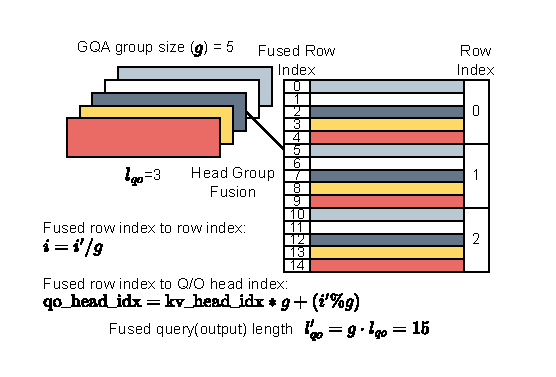
\includegraphics[width=0.5\textwidth]{figures/gqa-mapping.pdf}
    \caption{\sys's head-group fusion of query heads with the query length dimension in GQA.}
    \label{fig:flashinfer-gqa-packing}
\end{figure}

We prefer head-group fusion primarily for short query lengths. When the query length is sufficiently large, the query dimension itself yields enough workload to effectively utilize the KV-Cache, making head-group fusion less critical. Similar ideas have also been explored in other frameworks, such as XQA~\cite{xqa} in TensorRT-LLM~\cite{nvidia2023tensorrt}.

\section{Overhead of Sparse Gathering}
\label{sec:overhead-sparse-gathering}

In Section~\ref{sec:sparse-loading}, we detailed the design of \sys's sparse loading module, which transfers sparse rows from global memory into contiguous shared memory. Here, we measure the performance overhead associated with sparse gathering in \sys for both \emph{decode} and \emph{prefill} kernels.

\begin{figure}[ht]
    \centering
    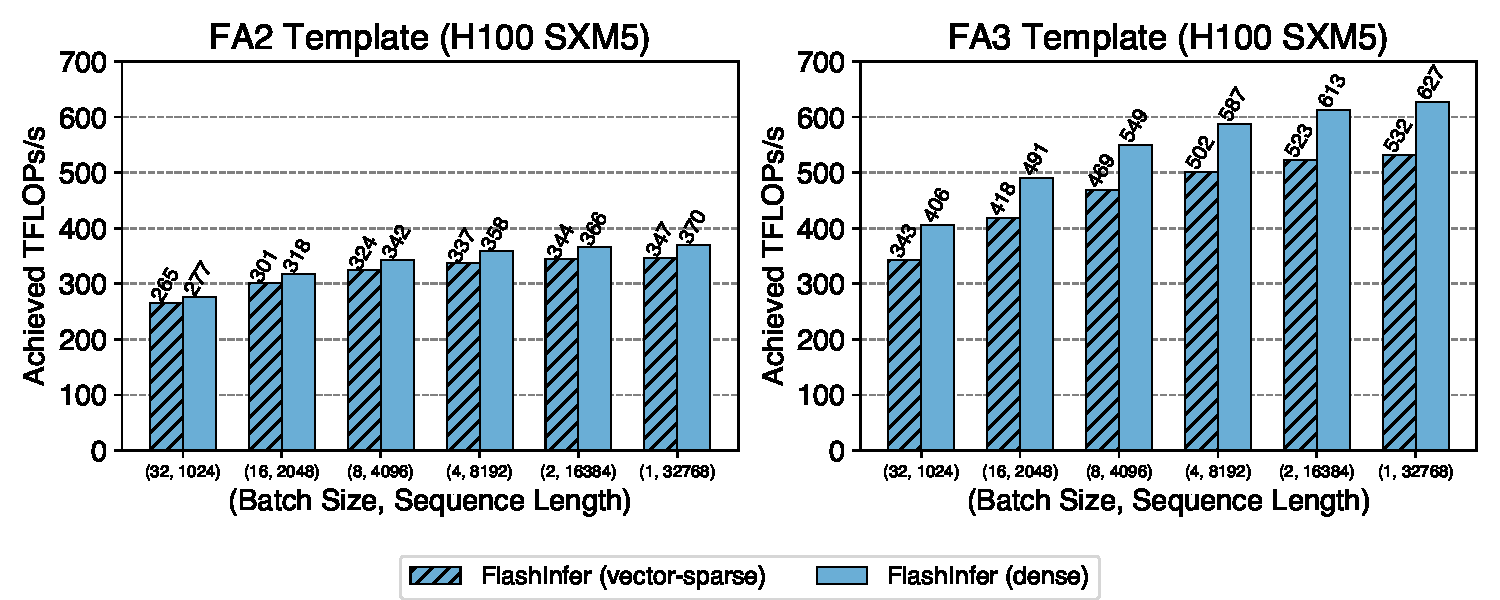
\includegraphics[width=0.4\textwidth]{figures/prefill-sparse-dense.pdf}
    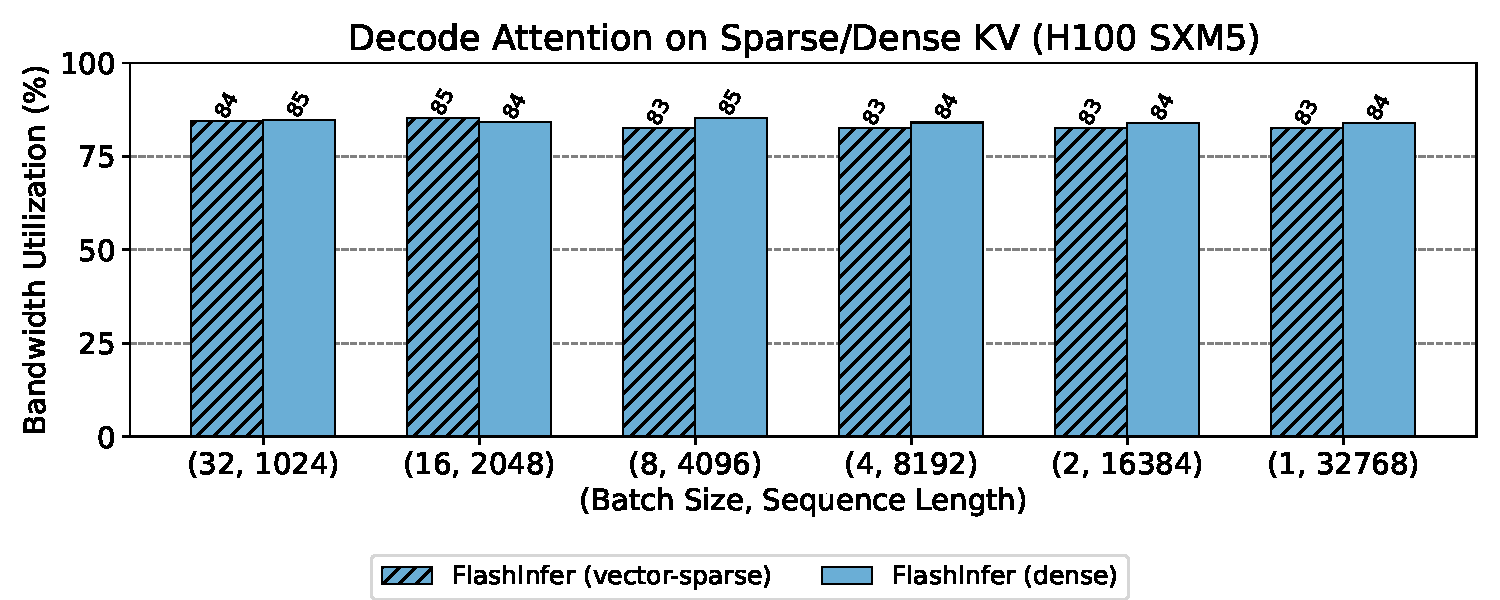
\includegraphics[width=0.4\textwidth]{figures/decode-sparse-dense.pdf}
    \caption{\textbf{Top:} Achieved TFLOPs/s for (causal) prefill attention kernels on FA2/FA3 templates with both dense/sparse KV-Cache. 
    \textbf{Bottom:} Achieved bandwidth utilization for decode attention kernels for both dense/sparse KV-Cache. 
    We use PageAttention with page size 1 (vector-sparse) for sparse KV-Cache. The x-axis shows various batch sizes and sequence lengths.}
    \label{fig:sparse-dense}
\end{figure}

Figure~\ref{fig:sparse-dense} compares achieved throughput in both prefill and decode kernels for sparse and dense (contiguous) KV-Cache.
For the prefill kernels, we measure the \textit{causal} attention scenario, which is common in LLM serving. For contiguous KV-Cache, We use the variable-length RaggedTensor prefill attention API\footnote{\url{https://docs.flashinfer.ai/api/prefill.html\#flashinfer.prefill.BatchPrefillWithRaggedKVCacheWrapper}}. For sparse KV-Cache, we use the PagedKVCache prefill attention API\footnote{\url{https://docs.flashinfer.ai/api/prefill.html\#flashinfer.prefill.BatchPrefillWithPagedKVCacheWrapper}}.

The number of query heads and KV heads are both fixed at 32, head dimension is set to 128. We vary batch size and sequence length to measure the achieved throughput. For decode kernels, the performance gap between sparse and dense KV-Cache is negligible (within $1\%$). For prefill kernels, there is approximately a $10\%$ performance gap.

Note that dense attention in the FA3 template uses TMA instructions (Tensor Memory Access) for key/value loading, which is unavailable for sparse gathering because Hopper Architecture's TMA only supports fixed-stride accesses, whereas sparse gathering requires arbitrary row indices. Consequently, sparse gathering on FA3 relies on Ampere-style asynchronous copy instructions and manual pointer arithmetic. This approach consumes more registers and necessitates smaller KV-tile size to avoid register spilling, leading to a slightly larger performance gap. By contrast, in the FA2 template (where both sparse and dense use Ampere's async-copy), the gap is smaller because the same tile size is used.

When the block column size in a block-sparse matrix is large (e.g., 128 or greater), TMA can be used for sparse gathering since each TMA instruction operates within a single block with fixed stride. We leave this optimization for future work. However, increasing the block column size reduces the flexibility of the block-sparse format, which might not be suitable for all use cases.

\section{The Choice of Backend}
\label{sec:backend-choice}

For NVIDIA GPUs, we build \sys on top of CUDA/CUTLASS~\cite{cutlass} instead of Triton~\cite{triton} for the following reasons:
\begin{enumerate}
    \item \textbf{Advanced NVIDIA GPU Features.} CUTLASS supports specialized GPU capabilities such as warp-specialization~\cite{warp-specialization} and TMA instructions~\cite{hopper-tma}, which are experimental or unsupported in Triton at this moment.
    \item \textbf{Fine-Grained Kernel Optimization.} While Triton provides tile-level abstractions, CUDA/CUTLASS affords finer control over thread-level registers. This flexibility simplifies incorporating low-level optimizations (e.g., PTX intrinsics) directly into our JIT templates, which is more challenging in Triton.
\end{enumerate}

Our load-balancing scheduler design (Section~\ref{sec:load-balanced-scheduling}) is largely backend-agnostic, allowing us to potentially integrate Triton in future versions of \sys and to adapt our approach to other hardware platforms.

\section{Memory Management}
\label{sec:memory-mgmt}

\sys manages a page-locked (pinned) host buffer and a device workspace buffer to store scheduler metadata and split-k partial outputs. We divide the device workspace buffer into \emph{sections}, each corresponding to an array of either scheduler metadata or partial split-k outputs. For each \lstinline{plan} call in the scheduler, we compute the scheduler metadata on the pinned host buffer and then issue a \lstinline{cudaMemcpyAsync} to transfer this data into the corresponding sections of the device workspace buffer.

\subsection{CUDAGraph-Compatible Workspace Layout}
\label{sec:cudagraph-compatible-layout}

Once a kernel is captured by CUDA Graph, its arguments (pointers and scalars) become fixed, implying that each section of the device workspace buffer must maintain a consistent address for the entire captured graph's lifetime. Therefore, we allocate the workspace buffer to its maximum required capacity for each section, based on upper-bound estimations of scheduler metadata and partial outputs.

\subsection{Split-K Writethrough Optimizations}
\label{sec:writethrough-optimizations}

In \sys's load-balancing scheduler (Section~\ref{sec:load-balanced-scheduling}), KV-splitting is only applied to requests that have large KV lengths. Requests with short KV lengths do not require splitting and hence have no reduction step from partial output. To save both computation and workspace memory, these small requests can write their partial outputs directly to the final output buffer (bypassing the device workspace buffer). This approach reduces both the required workspace size and the computational load within the contraction kernel.

\subsection{Workspace Buffer Size Estimation}
\label{sec:workspace-buffer-size}

The workspace buffer size depends on two main factors: 
(1) the required space for scheduler metadata, and 
(2) the required space for storing partial split-k outputs.

\paragraph{Scheduler Metadata.} The maximum size of each metadata section is derived from the largest possible number of concurrent requests and the maximum accumulated request length. Users must provide these upper bounds during the scheduler's first planning stage.

\paragraph{Partial Outputs.} The size of partial outputs depends on both the problem dimensions (i.e., the number of heads and the head dimension) and the number of CTAs per kernel launch. In our load-balancing algorithm~\ref{sec:load-balanced-scheduling}, only requests deemed ``long'' -- those whose KV length exceeds the total KV length divided by the number of CTAs -- are split. According to the Writethrough Optimizations in Section~\ref{sec:writethrough-optimizations}, only these split requests produce outputs in the workspace buffer. Because the number of splits cannot exceed the total number of CTAs, and each split yields at most two tiles that must be merged, there are at most \(2 \times \#\text{CTA}\) partial outputs. Each tile produces a partial output of size \(T_q \cdot H_{qo} \cdot (D + 1) \), where \(T_q\) is the query tile size, \(H_{qo}\) is the number of heads, and \(D+1\) is the head dimension and LSE dimension. Therefore, the upper bound for the total partial output size is:
\[
  2\,\#\text{CTA} \times T_q \times H_{qo} \times (D + 1).
\]
By default, the total number of CTAs is set to $k \times \#\text{SM}$, where $\#\text{SM}$ denotes the number of streaming multiprocessors on the GPU and $k$ is chosen to maximize CTA-level occupancy.
For tensor-core based microkernels with high register usage, $k$ typically does not exceed 2 on Ampere, and it is often 1 on Hopper (one CTA per SM, also referred to as a persistent kernel).

\section{Overlap of Attention with Other Operations}
\label{sec:overlap-attention}

Nanoflow~\cite{zhu2024nanoflow} overlaps GEMM, attention, and inter-device communication in separate CUDA streams, assigning a fixed number of SMs to each operation. In \sys, this SM number can be provided by the user through the plan functions, and the \sys load-balancing scheduler will allocate tiles accordingly.

\section{FP8--FP16 Mixed-Precision Attention}
\label{sec:mixed-precision}

Recent LLMs frequently adopt \texttt{fp8} KV-Cache to reduce memory bandwidth and storage costs~\cite{micikevicius2022fp8}. In \sys, we implement \emph{mixed-precision} attention kernels wherein the query and output remain in \texttt{fp16}, while the KV-Cache is stored in \texttt{fp8}. We leverage the fast numerical array converter and fragment shuffler proposed by \citet{gupta2024mixed} to accelerate dequantization and handle bitwidth mismatches efficiently. This design allows for reduced memory footprints and higher bandwidth utilization without significantly compromising numerical accuracy.


\section{Additional Evaluation}
\label{sec:additional-evaluation}

In this section, we present additional evaluation results to further validate the performance, scalability, and robustness of \sys across diverse experimental conditions.

\subsection{Comparison with FlexAttention}

We compare \sys and FlexAttention~\cite{he2024flexattention} on different attention variants using the AttentionGym~\cite{AttentionGym} benchmark on NVIDIA H100 80GB SXM.
We evaluated with batch size $16$, number of heads $16$ and head dim $128$, the CUDA version and the Triton version were fixed to 12.4 and 3.2, respectivelyrespectively.
Tables \ref{table:flexattention-causal-attn} to \ref{table:flexattention-sliding-window} show the performance of \sys and FlexAttention in TFLOPS/s, where higher numbers mean better performance.
Across all four scenarios and a range of sequence lengths, \sys consistently outperforms FlexAttention, with especially large gains at longer sequence lengths.
The better performance is mainly due to the usage of Hopper microarchitecture’s advanced features (such as warp specialization and TMA), and CUTLASS’s fine-grained resource control (at register-level rather than tile-level) over Triton. Note that these gaps will be alleviated once Triton fully supports these features.

\begin{table}[h]
\centering
\caption{Causal Attention}
\label{table:flexattention-causal-attn}
\begin{tabular}{lrr}
\toprule
Seq Length & FlexAttention & \sys \\
\midrule
512   & 209.11 & \textbf{250.454} \\
1024  & 294.53 & \textbf{406.554} \\
2048  & 376.90 & \textbf{487.236} \\
4096  & 421.00 & \textbf{548.388} \\
8192  & 441.26 & \textbf{587.903} \\
16384 & 453.57 & \textbf{612.259} \\
\bottomrule
\end{tabular}
\end{table}

\begin{table}[ht]
\centering
\vspace{-10pt}
\caption{Attention with Logits SoftCap}
\label{table:flexattention-logits-softcap}
\begin{tabular}{lrr}
\toprule
Seq Length & FlexAttention & \sys \\
\midrule
512   & 241.51 & \textbf{336.487} \\
1024  & 327.50 & \textbf{409.534} \\
2048  & 379.57 & \textbf{468.769} \\
4096  & 403.39 & \textbf{489.667} \\
8192  & 407.82 & \textbf{515.573} \\
16384 & 409.89 & \textbf{520.935} \\
\bottomrule
\end{tabular}
\end{table}

\begin{table}[ht]
\centering
\caption{ALiBi Bias~\cite{press2022alibi}}
\label{table:flexattention-alibi}
\begin{tabular}{lrr}
\toprule
Seq Length & FlexAttention & \sys \\
\midrule
512   & 253.22 & \textbf{403.899} \\
1024  & 344.70 & \textbf{500.220} \\
2048  & 406.14 & \textbf{535.498} \\
4096  & 426.13 & \textbf{561.324} \\
8192  & 436.35 & \textbf{573.493} \\
16384 & 434.86 & \textbf{578.005} \\
\bottomrule
\end{tabular}
\end{table}

\begin{table}[ht]
\centering
\vspace{-3pt}
\caption{Sliding Window (window size = $1024$)}
\label{table:flexattention-sliding-window}
\begin{tabular}{lrr}
\toprule
Seq Length & FlexAttention & \sys \\
\midrule
512   & 206.51 & \textbf{236.363} \\
1024  & 292.25 & \textbf{374.108} \\
2048  & 350.91 & \textbf{381.464} \\
4096  & 368.45 & \textbf{384.998} \\
8192  & 373.25 & \textbf{384.514} \\
16384 & 367.91 & \textbf{380.506} \\
\bottomrule
\end{tabular}
\end{table}


\subsection{Evaluation of Shared-Prefix Attention Kernels}

We measure shared-prefix attention kernels with suffix length $128$.
Table~\ref{table:eval-shared-prefix-attn} shows the kernel latency under different shared prefix lengths, scenarios and batch sizes, where numbers are in microseconds (us), and ``composable'' means composable format while ``single'' means single format.
The composable format benefits long prefixes (e.g., 32k) and large batch sizes (e.g., $64$).
However, these speedups do not always yield proportional end-to-end gains because real-world shared prefix sizes tend to be smaller.

\begin{table}[hbt]
\small
\centering
\caption{Latency of Shared-Prefix Attention Kernels}
\label{table:eval-shared-prefix-attn}
\begin{tabular}{lr@{}r@{}r@{}r@{}}
\toprule
\makecell{Shared \\ Prefix \\ Length} & \makecell{Composable \\ (BS=16)} & \makecell{Single \\ (BS=16)} & \makecell{Composable \\ (BS=64)} & \makecell{Single \\ (BS=64)} \\
\midrule
1024   & \textbf{45.17}  & 46.52  & 87.86   & 130.49 \\
8192   & \textbf{88.67}  & 226.57 & 125.76  & 931.75 \\
32768  & \textbf{217.42} & 945.67 & 254.54  & 4090   \\
\bottomrule
\end{tabular}
\end{table}

\subsection{Ablation Study on Variable Sequence Length and load-balancing scheduler}

We conduct ablations on the effect of load-balancing scheduler~(Section~\ref{sec:load-balanced-scheduling}).
Table~\ref{table:eval-ablation-itl} and~\ref{table:eval-ablation-ttft} show the results for Llama 3.1-8B-Instruct running on an NVIDIA H100 SXM5 GPU with SGLang~\cite{zheng2023sglang} + \sys (with and without load-balancing scheduler).
We evaluate the inter-token latency (ITL, ms) and time-to-first-token (TTFT, ms) with three datasets: ShareGPT, variable sequence length with input lengths sampled from $U(512, 2048)$ and output fixed at $256$, and variable sequence length with input lengths sampled from $U(4096, 16384)$ and output fixed at $256$. ``RR'' in the tables means request rate.

\begin{table}[hbt]
\small
\centering
\vspace{-5pt}
\caption{Load-balancing Scheduler Ablation Study (ITL)}
\label{table:eval-ablation-itl}
\begin{tabular}{@{}lrrr@{}}
\toprule
Scenario & \makecell{w/ \\ Load- \\ Balancing} & \makecell{w/o \\ Load- \\ Balancing} & Triton \\
\midrule
ShareGPT (RR=16) & \textbf{8.96} & 9.16 & 9.36 \\
$U(512, 2048)$ (RR=8)        & \textbf{8.21} & 8.42 & 8.49 \\
$U(4096, 16384)$ (RR=1)        & \textbf{8.63} & 13.89 & 11.08 \\
\bottomrule
\end{tabular}
\end{table}

\begin{table}[hbt]
\small
\centering
\caption{Load-balancing Scheduler Ablation Study (TTFT)}
\label{table:eval-ablation-ttft}
\begin{tabular}{@{}lrrr@{}}
\toprule
Scenario & \makecell{w/ \\ Load- \\ Balancing} & \makecell{w/o \\ Load- \\ Balancing} & Triton \\
\midrule
ShareGPT (RR=16) & \textbf{39.05} & 39.42 & 52.92 \\
 $U(512, 2048)$ (RR=8)        & \textbf{66.78} & 67.38 & 68.48 \\
 $U(4096, 16384)$ (RR=1)        & \textbf{411.02} & 421.60 & 566.30 \\
\bottomrule
\end{tabular}
\end{table}

\subsection{vLLM Integration Evaluation}

We compare the vLLM with \sys backend and its default backend with a fixed request rate of $16$, reporting throughput (tokens/s), inter-token latency (ITL, ms), and time-to-first-token (TTFT, ms) in Table~\ref{table:eval-vllm-integration}.
\sys reduces ITL by aroudn 13\% using fp8 KV-cache, but heavy Python overhead in vLLM integration (e.g. array operations) at host side causes minor regressions with bf16. Our future optimizations will address these in C++ and move the scheduler to device.

\begin{table}[hbt]
\centering
\caption{vLLM Integration Evaluation}
\label{table:eval-vllm-integration}
\begin{tabular}{@{}l@{}rrr@{}}
\toprule
Backend         & Throughput & \makecell{Median \\ ITL} & \makecell{Median \\ TTFT} \\
\midrule
Default (bf16)  & 6062.89    & 10.42      & 35.85      \\
\sys (bf16)    & 6065.41    & 10.63      & 36.60      \\
Default (e4m3)  & 6015.86    & 12.56      & 39.74      \\
\sys (e4m3)    & 6020.32    & 10.92      & 37.93      \\
\bottomrule
\end{tabular}
\end{table}

\subsection{Fine-Grained Block-Sparsity Evaluation}

\sys supports fine-grained block-sparse matrices, which is useful in many KV-Cache pruning algorithms.
We measure the kernel performance on Quest~\cite{tang2024quest}, a state-of-the-art long-context modeling algorithm, which uses fine-grained sparsity in KV-Cache.
We compared the batch decoding attention kernel in Quest using \sys and compared its performance to PyTorch SDPA and FlexAttention on an NVIDIA H100 SXM5 GPU with the configuration (block size 16, num\_qo\_heads $32$, num\_kv\_heads $32$, head\_dim $128$).
All latency values reported are in microseconds (us).

As shown in Table~\ref{table:eval-sparsity-flashinfer} to~\ref{table:eval-sparsity-flexattention}, \sys demonstrates a considerable performance advantage, achieving up to a 20x speedup for long sequence lengths.
Currently FlexAttention relies on large block size templates, while \sys employs a sparse-row gathering strategy to leverage dense tensor cores for small block sizes. This design choice supports fine-grained KV-cache pruning.

\begin{table}[hbt]
\small
\centering
\caption{\sys Fine-Grained Sparsity  Latency (us)}
\label{table:eval-sparsity-flashinfer}
\begin{tabular}{@{}lrrrr@{}}
\toprule
\multicolumn{1}{c}{} & \multicolumn{4}{c}{page\_budget} \\
\cmidrule(l){2-5}
seq\_len & 64 & 128 & 256 & 512 \\
\midrule
4096  & 20.299 & 30.361 & 44.383 & 44.430 \\
8192  & 22.273 & 28.603 & 44.928 & 68.194 \\
16384 & 20.485 & 28.678 & 44.677 & 68.700 \\
32768 & 22.371 & 28.700 & 44.988 & 68.478 \\
\bottomrule
\end{tabular}
\end{table}

\begin{table}[hbt]
\small
\centering
\caption{PyTorch SDPA Fine-Grained Sparsity Latency (us)}
\label{table:eval-sparsity-torch}
\begin{tabular}{@{}lrrrr@{}}
\toprule
\multicolumn{1}{c}{} & \multicolumn{4}{c}{page\_budget} \\
\cmidrule(l){2-5}
seq\_len & 64 & 128 & 256 & 512 \\
\midrule
4096  & 287.684 & 288.904 & 287.715 & 287.807 \\
8192  & 474.631 & 474.508 & 474.683 & 473.070 \\
16384 & 857.319 & 857.570 & 857.094 & 857.728 \\
32768 & 1711.955 & 1711.621 & 1713.093 & 1711.709 \\
\bottomrule
\end{tabular}
\end{table}

\begin{table}[hbt]
\small
\centering
\caption{FlexAttention Fine-Grained Sparsity Latency (us)}
\label{table:eval-sparsity-flexattention}
\begin{tabular}{@{}lrrrr@{}}
\toprule
\multicolumn{1}{c}{} & \multicolumn{4}{c}{page\_budget} \\
\cmidrule(l){2-5}
seq\_len & 64 & 128 & 256 & 512 \\
\midrule
4096  & 1100.349 & 1097.356 & 1073.753 & 1071.797 \\
8192  & 1092.695 & 1099.100 & 1078.081 & 1074.886 \\
16384 & 1109.817 & 1101.535 & 1077.639 & 1076.859 \\
32768 & 1169.109 & 1187.395 & 1176.332 & 1174.502 \\
\bottomrule
\end{tabular}
\end{table}